\documentclass{report}

%%%%%%%%%%%%%%%%%%%%%%%%%%%%%%%%%
% PACKAGE IMPORTS
%%%%%%%%%%%%%%%%%%%%%%%%%%%%%%%%%


\usepackage[tmargin=2cm,rmargin=1in,lmargin=1in,margin=0.85in,bmargin=2cm,footskip=.2in]{geometry}
\usepackage{amsmath,amsfonts,amsthm,amssymb,mathtools}
\usepackage[varbb]{newpxmath}
\usepackage{xfrac}
\usepackage[makeroom]{cancel}
\usepackage{mathtools}
\usepackage{bookmark}
\usepackage{enumitem}
\usepackage{hyperref,theoremref}
\hypersetup{
	pdftitle={Assignment},
	colorlinks=true, linkcolor=doc!90,
	bookmarksnumbered=true,
	bookmarksopen=true
}
\usepackage[most,many,breakable]{tcolorbox}
\usepackage{xcolor}
\usepackage{varwidth}
\usepackage{varwidth}
\usepackage{etoolbox}
%\usepackage{authblk}
\usepackage{nameref}
\usepackage{multicol,array}
\usepackage{tikz-cd}
\usepackage[ruled,vlined,linesnumbered]{algorithm2e}
\usepackage{comment} % enables the use of multi-line comments (\ifx \fi) 
\usepackage{import}
\usepackage{xifthen}
\usepackage{pdfpages}
\usepackage{transparent}
\usepackage{lmodern}

\newcommand\mycommfont[1]{\footnotesize\ttfamily\textcolor{blue}{#1}}
\SetCommentSty{mycommfont}
\newcommand{\incfig}[1]{%
    \def\svgwidth{\columnwidth}
    \import{./figures/}{#1.pdf_tex}
}

\usepackage{tikzsymbols}
\renewcommand\qedsymbol{$\Laughey$}


%\usepackage{import}
%\usepackage{xifthen}
%\usepackage{pdfpages}
%\usepackage{transparent}


%%%%%%%%%%%%%%%%%%%%%%%%%%%%%%
% SELF MADE COLORS
%%%%%%%%%%%%%%%%%%%%%%%%%%%%%%



\definecolor{myg}{RGB}{56, 140, 70}
\definecolor{myb}{RGB}{45, 111, 177}
\definecolor{myr}{RGB}{199, 68, 64}
\definecolor{mytheorembg}{HTML}{F2F2F9}
\definecolor{mytheoremfr}{HTML}{00007B}
\definecolor{mylenmabg}{HTML}{FFFAF8}
\definecolor{mylenmafr}{HTML}{983b0f}
\definecolor{mypropbg}{HTML}{f2fbfc}
\definecolor{mypropfr}{HTML}{191971}
\definecolor{myexamplebg}{HTML}{F2FBF8}
\definecolor{myexamplefr}{HTML}{88D6D1}
\definecolor{myexampleti}{HTML}{2A7F7F}
\definecolor{mydefinitbg}{HTML}{E5E5FF}
\definecolor{mydefinitfr}{HTML}{3F3FA3}
\definecolor{notesgreen}{RGB}{0,162,0}
\definecolor{myp}{RGB}{197, 92, 212}
\definecolor{mygr}{HTML}{2C3338}
\definecolor{myred}{RGB}{127,0,0}
\definecolor{myyellow}{RGB}{169,121,69}
\definecolor{myexercisebg}{HTML}{F2FBF8}
\definecolor{myexercisefg}{HTML}{88D6D1}


%%%%%%%%%%%%%%%%%%%%%%%%%%%%
% TCOLORBOX SETUPS
%%%%%%%%%%%%%%%%%%%%%%%%%%%%

\setlength{\parindent}{1cm}
%================================
% THEOREM BOX
%================================

\tcbuselibrary{theorems,skins,hooks}
\newtcbtheorem[number within=section]{Theorem}{Theorem}
{%
	enhanced,
	breakable,
	colback = mytheorembg,
	frame hidden,
	boxrule = 0sp,
	borderline west = {2pt}{0pt}{mytheoremfr},
	sharp corners,
	detach title,
	before upper = \tcbtitle\par\smallskip,
	coltitle = mytheoremfr,
	fonttitle = \bfseries\sffamily,
	description font = \mdseries,
	separator sign none,
	segmentation style={solid, mytheoremfr},
}
{th}

\tcbuselibrary{theorems,skins,hooks}
\newtcbtheorem[number within=chapter]{theorem}{Theorem}
{%
	enhanced,
	breakable,
	colback = mytheorembg,
	frame hidden,
	boxrule = 0sp,
	borderline west = {2pt}{0pt}{mytheoremfr},
	sharp corners,
	detach title,
	before upper = \tcbtitle\par\smallskip,
	coltitle = mytheoremfr,
	fonttitle = \bfseries\sffamily,
	description font = \mdseries,
	separator sign none,
	segmentation style={solid, mytheoremfr},
}
{th}


\tcbuselibrary{theorems,skins,hooks}
\newtcolorbox{Theoremcon}
{%
	enhanced
	,breakable
	,colback = mytheorembg
	,frame hidden
	,boxrule = 0sp
	,borderline west = {2pt}{0pt}{mytheoremfr}
	,sharp corners
	,description font = \mdseries
	,separator sign none
}

%================================
% Corollery
%================================
\tcbuselibrary{theorems,skins,hooks}
\newtcbtheorem[number within=section]{Corollary}{Corollary}
{%
	enhanced
	,breakable
	,colback = myp!10
	,frame hidden
	,boxrule = 0sp
	,borderline west = {2pt}{0pt}{myp!85!black}
	,sharp corners
	,detach title
	,before upper = \tcbtitle\par\smallskip
	,coltitle = myp!85!black
	,fonttitle = \bfseries\sffamily
	,description font = \mdseries
	,separator sign none
	,segmentation style={solid, myp!85!black}
}
{th}
\tcbuselibrary{theorems,skins,hooks}
\newtcbtheorem[number within=chapter]{corollary}{Corollary}
{%
	enhanced
	,breakable
	,colback = myp!10
	,frame hidden
	,boxrule = 0sp
	,borderline west = {2pt}{0pt}{myp!85!black}
	,sharp corners
	,detach title
	,before upper = \tcbtitle\par\smallskip
	,coltitle = myp!85!black
	,fonttitle = \bfseries\sffamily
	,description font = \mdseries
	,separator sign none
	,segmentation style={solid, myp!85!black}
}
{th}


%================================
% LENMA
%================================

\tcbuselibrary{theorems,skins,hooks}
\newtcbtheorem[number within=section]{Lenma}{Lenma}
{%
	enhanced,
	breakable,
	colback = mylenmabg,
	frame hidden,
	boxrule = 0sp,
	borderline west = {2pt}{0pt}{mylenmafr},
	sharp corners,
	detach title,
	before upper = \tcbtitle\par\smallskip,
	coltitle = mylenmafr,
	fonttitle = \bfseries\sffamily,
	description font = \mdseries,
	separator sign none,
	segmentation style={solid, mylenmafr},
}
{th}

\tcbuselibrary{theorems,skins,hooks}
\newtcbtheorem[number within=chapter]{lenma}{Lenma}
{%
	enhanced,
	breakable,
	colback = mylenmabg,
	frame hidden,
	boxrule = 0sp,
	borderline west = {2pt}{0pt}{mylenmafr},
	sharp corners,
	detach title,
	before upper = \tcbtitle\par\smallskip,
	coltitle = mylenmafr,
	fonttitle = \bfseries\sffamily,
	description font = \mdseries,
	separator sign none,
	segmentation style={solid, mylenmafr},
}
{th}


%================================
% PROPOSITION
%================================

\tcbuselibrary{theorems,skins,hooks}
\newtcbtheorem[number within=section]{Prop}{Proposition}
{%
	enhanced,
	breakable,
	colback = mypropbg,
	frame hidden,
	boxrule = 0sp,
	borderline west = {2pt}{0pt}{mypropfr},
	sharp corners,
	detach title,
	before upper = \tcbtitle\par\smallskip,
	coltitle = mypropfr,
	fonttitle = \bfseries\sffamily,
	description font = \mdseries,
	separator sign none,
	segmentation style={solid, mypropfr},
}
{th}

\tcbuselibrary{theorems,skins,hooks}
\newtcbtheorem[number within=chapter]{prop}{Proposition}
{%
	enhanced,
	breakable,
	colback = mypropbg,
	frame hidden,
	boxrule = 0sp,
	borderline west = {2pt}{0pt}{mypropfr},
	sharp corners,
	detach title,
	before upper = \tcbtitle\par\smallskip,
	coltitle = mypropfr,
	fonttitle = \bfseries\sffamily,
	description font = \mdseries,
	separator sign none,
	segmentation style={solid, mypropfr},
}
{th}


%================================
% CLAIM
%================================

\tcbuselibrary{theorems,skins,hooks}
\newtcbtheorem[number within=section]{claim}{Claim}
{%
	enhanced
	,breakable
	,colback = myg!10
	,frame hidden
	,boxrule = 0sp
	,borderline west = {2pt}{0pt}{myg}
	,sharp corners
	,detach title
	,before upper = \tcbtitle\par\smallskip
	,coltitle = myg!85!black
	,fonttitle = \bfseries\sffamily
	,description font = \mdseries
	,separator sign none
	,segmentation style={solid, myg!85!black}
}
{th}



%================================
% Exercise
%================================

\tcbuselibrary{theorems,skins,hooks}
\newtcbtheorem[number within=section]{Exercise}{Exercise}
{%
	enhanced,
	breakable,
	colback = myexercisebg,
	frame hidden,
	boxrule = 0sp,
	borderline west = {2pt}{0pt}{myexercisefg},
	sharp corners,
	detach title,
	before upper = \tcbtitle\par\smallskip,
	coltitle = myexercisefg,
	fonttitle = \bfseries\sffamily,
	description font = \mdseries,
	separator sign none,
	segmentation style={solid, myexercisefg},
}
{th}

\tcbuselibrary{theorems,skins,hooks}
\newtcbtheorem[number within=chapter]{exercise}{Exercise}
{%
	enhanced,
	breakable,
	colback = myexercisebg,
	frame hidden,
	boxrule = 0sp,
	borderline west = {2pt}{0pt}{myexercisefg},
	sharp corners,
	detach title,
	before upper = \tcbtitle\par\smallskip,
	coltitle = myexercisefg,
	fonttitle = \bfseries\sffamily,
	description font = \mdseries,
	separator sign none,
	segmentation style={solid, myexercisefg},
}
{th}

%================================
% EXAMPLE BOX
%================================

\newtcbtheorem[number within=section]{Example}{Example}
{%
	colback = myexamplebg
	,breakable
	,colframe = myexamplefr
	,coltitle = myexampleti
	,boxrule = 1pt
	,sharp corners
	,detach title
	,before upper=\tcbtitle\par\smallskip
	,fonttitle = \bfseries
	,description font = \mdseries
	,separator sign none
	,description delimiters parenthesis
}
{ex}

\newtcbtheorem[number within=chapter]{example}{Example}
{%
	colback = myexamplebg
	,breakable
	,colframe = myexamplefr
	,coltitle = myexampleti
	,boxrule = 1pt
	,sharp corners
	,detach title
	,before upper=\tcbtitle\par\smallskip
	,fonttitle = \bfseries
	,description font = \mdseries
	,separator sign none
	,description delimiters parenthesis
}
{ex}

%================================
% DEFINITION BOX
%================================

\newtcbtheorem[number within=section]{Definition}{Definition}{enhanced,
	before skip=2mm,after skip=2mm, colback=red!5,colframe=red!80!black,boxrule=0.5mm,
	attach boxed title to top left={xshift=1cm,yshift*=1mm-\tcboxedtitleheight}, varwidth boxed title*=-3cm,
	boxed title style={frame code={
					\path[fill=tcbcolback]
					([yshift=-1mm,xshift=-1mm]frame.north west)
					arc[start angle=0,end angle=180,radius=1mm]
					([yshift=-1mm,xshift=1mm]frame.north east)
					arc[start angle=180,end angle=0,radius=1mm];
					\path[left color=tcbcolback!60!black,right color=tcbcolback!60!black,
						middle color=tcbcolback!80!black]
					([xshift=-2mm]frame.north west) -- ([xshift=2mm]frame.north east)
					[rounded corners=1mm]-- ([xshift=1mm,yshift=-1mm]frame.north east)
					-- (frame.south east) -- (frame.south west)
					-- ([xshift=-1mm,yshift=-1mm]frame.north west)
					[sharp corners]-- cycle;
				},interior engine=empty,
		},
	fonttitle=\bfseries,
	title={#2},#1}{def}
\newtcbtheorem[number within=chapter]{definition}{Definition}{enhanced,
	before skip=2mm,after skip=2mm, colback=red!5,colframe=red!80!black,boxrule=0.5mm,
	attach boxed title to top left={xshift=1cm,yshift*=1mm-\tcboxedtitleheight}, varwidth boxed title*=-3cm,
	boxed title style={frame code={
					\path[fill=tcbcolback]
					([yshift=-1mm,xshift=-1mm]frame.north west)
					arc[start angle=0,end angle=180,radius=1mm]
					([yshift=-1mm,xshift=1mm]frame.north east)
					arc[start angle=180,end angle=0,radius=1mm];
					\path[left color=tcbcolback!60!black,right color=tcbcolback!60!black,
						middle color=tcbcolback!80!black]
					([xshift=-2mm]frame.north west) -- ([xshift=2mm]frame.north east)
					[rounded corners=1mm]-- ([xshift=1mm,yshift=-1mm]frame.north east)
					-- (frame.south east) -- (frame.south west)
					-- ([xshift=-1mm,yshift=-1mm]frame.north west)
					[sharp corners]-- cycle;
				},interior engine=empty,
		},
	fonttitle=\bfseries,
	title={#2},#1}{def}



%================================
% Solution BOX
%================================

\makeatletter
\newtcbtheorem{question}{Question}{enhanced,
	breakable,
	colback=white,
	colframe=myb!80!black,
	attach boxed title to top left={yshift*=-\tcboxedtitleheight},
	fonttitle=\bfseries,
	title={#2},
	boxed title size=title,
	boxed title style={%
			sharp corners,
			rounded corners=northwest,
			colback=tcbcolframe,
			boxrule=0pt,
		},
	underlay boxed title={%
			\path[fill=tcbcolframe] (title.south west)--(title.south east)
			to[out=0, in=180] ([xshift=5mm]title.east)--
			(title.center-|frame.east)
			[rounded corners=\kvtcb@arc] |-
			(frame.north) -| cycle;
		},
	#1
}{def}
\makeatother

%================================
% SOLUTION BOX
%================================

\makeatletter
\newtcolorbox{solution}{enhanced,
	breakable,
	colback=white,
	colframe=myg!80!black,
	attach boxed title to top left={yshift*=-\tcboxedtitleheight},
	title=Solution,
	boxed title size=title,
	boxed title style={%
			sharp corners,
			rounded corners=northwest,
			colback=tcbcolframe,
			boxrule=0pt,
		},
	underlay boxed title={%
			\path[fill=tcbcolframe] (title.south west)--(title.south east)
			to[out=0, in=180] ([xshift=5mm]title.east)--
			(title.center-|frame.east)
			[rounded corners=\kvtcb@arc] |-
			(frame.north) -| cycle;
		},
}
\makeatother

%================================
% Question BOX
%================================

\makeatletter
\newtcbtheorem{qstion}{Question}{enhanced,
	breakable,
	colback=white,
	colframe=mygr,
	attach boxed title to top left={yshift*=-\tcboxedtitleheight},
	fonttitle=\bfseries,
	title={#2},
	boxed title size=title,
	boxed title style={%
			sharp corners,
			rounded corners=northwest,
			colback=tcbcolframe,
			boxrule=0pt,
		},
	underlay boxed title={%
			\path[fill=tcbcolframe] (title.south west)--(title.south east)
			to[out=0, in=180] ([xshift=5mm]title.east)--
			(title.center-|frame.east)
			[rounded corners=\kvtcb@arc] |-
			(frame.north) -| cycle;
		},
	#1
}{def}
\makeatother

\newtcbtheorem[number within=chapter]{wconc}{Wrong Concept}{
	breakable,
	enhanced,
	colback=white,
	colframe=myr,
	arc=0pt,
	outer arc=0pt,
	fonttitle=\bfseries\sffamily\large,
	colbacktitle=myr,
	attach boxed title to top left={},
	boxed title style={
			enhanced,
			skin=enhancedfirst jigsaw,
			arc=3pt,
			bottom=0pt,
			interior style={fill=myr}
		},
	#1
}{def}



%================================
% NOTE BOX
%================================

\usetikzlibrary{arrows,calc,shadows.blur}
\tcbuselibrary{skins}
\newtcolorbox{note}[1][]{%
	enhanced jigsaw,
	colback=gray!20!white,%
	colframe=gray!80!black,
	size=small,
	boxrule=1pt,
	title=\textbf{Note:-},
	halign title=flush center,
	coltitle=black,
	breakable,
	drop shadow=black!50!white,
	attach boxed title to top left={xshift=1cm,yshift=-\tcboxedtitleheight/2,yshifttext=-\tcboxedtitleheight/2},
	minipage boxed title=1.5cm,
	boxed title style={%
			colback=white,
			size=fbox,
			boxrule=1pt,
			boxsep=2pt,
			underlay={%
					\coordinate (dotA) at ($(interior.west) + (-0.5pt,0)$);
					\coordinate (dotB) at ($(interior.east) + (0.5pt,0)$);
					\begin{scope}
						\clip (interior.north west) rectangle ([xshift=3ex]interior.east);
						\filldraw [white, blur shadow={shadow opacity=60, shadow yshift=-.75ex}, rounded corners=2pt] (interior.north west) rectangle (interior.south east);
					\end{scope}
					\begin{scope}[gray!80!black]
						\fill (dotA) circle (2pt);
						\fill (dotB) circle (2pt);
					\end{scope}
				},
		},
	#1,
}

%%%%%%%%%%%%%%%%%%%%%%%%%%%%%%
% SELF MADE COMMANDS
%%%%%%%%%%%%%%%%%%%%%%%%%%%%%%


\newcommand{\thm}[2]{\begin{Theorem}{#1}{}#2\end{Theorem}}
\newcommand{\cor}[2]{\begin{Corollary}{#1}{}#2\end{Corollary}}
\newcommand{\mlenma}[2]{\begin{Lenma}{#1}{}#2\end{Lenma}}
\newcommand{\mprop}[2]{\begin{Prop}{#1}{}#2\end{Prop}}
\newcommand{\clm}[3]{\begin{claim}{#1}{#2}#3\end{claim}}
\newcommand{\wc}[2]{\begin{wconc}{#1}{}\setlength{\parindent}{1cm}#2\end{wconc}}
\newcommand{\thmcon}[1]{\begin{Theoremcon}{#1}\end{Theoremcon}}
\newcommand{\ex}[2]{\begin{Example}{#1}{}#2\end{Example}}
\newcommand{\dfn}[2]{\begin{Definition}[colbacktitle=red!75!black]{#1}{}#2\end{Definition}}
\newcommand{\dfnc}[2]{\begin{definition}[colbacktitle=red!75!black]{#1}{}#2\end{definition}}
\newcommand{\qs}[2]{\begin{question}{#1}{}#2\end{question}}
\newcommand{\pf}[2]{\begin{myproof}[#1]#2\end{myproof}}
\newcommand{\nt}[1]{\begin{note}#1\end{note}}

\newcommand*\circled[1]{\tikz[baseline=(char.base)]{
		\node[shape=circle,draw,inner sep=1pt] (char) {#1};}}
\newcommand\getcurrentref[1]{%
	\ifnumequal{\value{#1}}{0}
	{??}
	{\the\value{#1}}%
}
\newcommand{\getCurrentSectionNumber}{\getcurrentref{section}}
\newenvironment{myproof}[1][\proofname]{%
	\proof[\bfseries #1: ]%
}{\endproof}

\newcommand{\mclm}[2]{\begin{myclaim}[#1]#2\end{myclaim}}
\newenvironment{myclaim}[1][\claimname]{\proof[\bfseries #1: ]}{}

\newcounter{mylabelcounter}

\makeatletter
\newcommand{\setword}[2]{%
	\phantomsection
	#1\def\@currentlabel{\unexpanded{#1}}\label{#2}%
}
\makeatother




\tikzset{
	symbol/.style={
			draw=none,
			every to/.append style={
					edge node={node [sloped, allow upside down, auto=false]{$#1$}}}
		}
}


% deliminators
\DeclarePairedDelimiter{\abs}{\lvert}{\rvert}
\DeclarePairedDelimiter{\norm}{\lVert}{\rVert}

\DeclarePairedDelimiter{\ceil}{\lceil}{\rceil}
\DeclarePairedDelimiter{\floor}{\lfloor}{\rfloor}
\DeclarePairedDelimiter{\round}{\lfloor}{\rceil}

\newsavebox\diffdbox
\newcommand{\slantedromand}{{\mathpalette\makesl{d}}}
\newcommand{\makesl}[2]{%
\begingroup
\sbox{\diffdbox}{$\mathsurround=0pt#1\mathrm{#2}$}%
\pdfsave
\pdfsetmatrix{1 0 0.2 1}%
\rlap{\usebox{\diffdbox}}%
\pdfrestore
\hskip\wd\diffdbox
\endgroup
}
\newcommand{\dd}[1][]{\ensuremath{\mathop{}\!\ifstrempty{#1}{%
\slantedromand\@ifnextchar^{\hspace{0.2ex}}{\hspace{0.1ex}}}%
{\slantedromand\hspace{0.2ex}^{#1}}}}
\ProvideDocumentCommand\dv{o m g}{%
  \ensuremath{%
    \IfValueTF{#3}{%
      \IfNoValueTF{#1}{%
        \frac{\dd #2}{\dd #3}%
      }{%
        \frac{\dd^{#1} #2}{\dd #3^{#1}}%
      }%
    }{%
      \IfNoValueTF{#1}{%
        \frac{\dd}{\dd #2}%
      }{%
        \frac{\dd^{#1}}{\dd #2^{#1}}%
      }%
    }%
  }%
}
\providecommand*{\pdv}[3][]{\frac{\partial^{#1}#2}{\partial#3^{#1}}}
%  - others
\DeclareMathOperator{\Lap}{\mathcal{L}}
\DeclareMathOperator{\Var}{Var} % varience
\DeclareMathOperator{\Cov}{Cov} % covarience
\DeclareMathOperator{\E}{E} % expected

% Since the amsthm package isn't loaded

% I prefer the slanted \leq
\let\oldleq\leq % save them in case they're every wanted
\let\oldgeq\geq
\renewcommand{\leq}{\leqslant}
\renewcommand{\geq}{\geqslant}

% % redefine matrix env to allow for alignment, use r as default
% \renewcommand*\env@matrix[1][r]{\hskip -\arraycolsep
%     \let\@ifnextchar\new@ifnextchar
%     \array{*\c@MaxMatrixCols #1}}


%\usepackage{framed}
%\usepackage{titletoc}
%\usepackage{etoolbox}
%\usepackage{lmodern}


%\patchcmd{\tableofcontents}{\contentsname}{\sffamily\contentsname}{}{}

%\renewenvironment{leftbar}
%{\def\FrameCommand{\hspace{6em}%
%		{\color{myyellow}\vrule width 2pt depth 6pt}\hspace{1em}}%
%	\MakeFramed{\parshape 1 0cm \dimexpr\textwidth-6em\relax\FrameRestore}\vskip2pt%
%}
%{\endMakeFramed}

%\titlecontents{chapter}
%[0em]{\vspace*{2\baselineskip}}
%{\parbox{4.5em}{%
%		\hfill\Huge\sffamily\bfseries\color{myred}\thecontentspage}%
%	\vspace*{-2.3\baselineskip}\leftbar\textsc{\small\chaptername~\thecontentslabel}\\\sffamily}
%{}{\endleftbar}
%\titlecontents{section}
%[8.4em]
%{\sffamily\contentslabel{3em}}{}{}
%{\hspace{0.5em}\nobreak\itshape\color{myred}\contentspage}
%\titlecontents{subsection}
%[8.4em]
%{\sffamily\contentslabel{3em}}{}{}  
%{\hspace{0.5em}\nobreak\itshape\color{myred}\contentspage}



%%%%%%%%%%%%%%%%%%%%%%%%%%%%%%%%%%%%%%%%%%%
% TABLE OF CONTENTS
%%%%%%%%%%%%%%%%%%%%%%%%%%%%%%%%%%%%%%%%%%%

\usepackage{tikz}
\definecolor{doc}{RGB}{0,60,110}
\usepackage{titletoc}
\contentsmargin{0cm}
\titlecontents{chapter}[3.7pc]
{\addvspace{30pt}%
	\begin{tikzpicture}[remember picture, overlay]%
		\draw[fill=doc!60,draw=doc!60] (-7,-.1) rectangle (-0.9,.5);%
		\pgftext[left,x=-3.5cm,y=0.2cm]{\color{white}\Large\sc\bfseries Chapter\ \thecontentslabel};%
	\end{tikzpicture}\color{doc!60}\large\sc\bfseries}%
{}
{}
{\;\titlerule\;\large\sc\bfseries Page \thecontentspage
	\begin{tikzpicture}[remember picture, overlay]
		\draw[fill=doc!60,draw=doc!60] (2pt,0) rectangle (4,0.1pt);
	\end{tikzpicture}}%
\titlecontents{section}[3.7pc]
{\addvspace{2pt}}
{\contentslabel[\thecontentslabel]{2pc}}
{}
{\hfill\small \thecontentspage}
[]
\titlecontents*{subsection}[3.7pc]
{\addvspace{-1pt}\small}
{}
{}
{\ --- \small\thecontentspage}
[ \textbullet\ ][]

\makeatletter
\renewcommand{\tableofcontents}{%
	\chapter*{%
	  \vspace*{-20\p@}%
	  \begin{tikzpicture}[remember picture, overlay]%
		  \pgftext[right,x=15cm,y=0.2cm]{\color{doc!60}\Huge\sc\bfseries \contentsname};%
		  \draw[fill=doc!60,draw=doc!60] (13,-.75) rectangle (20,1);%
		  \clip (13,-.75) rectangle (20,1);
		  \pgftext[right,x=15cm,y=0.2cm]{\color{white}\Huge\sc\bfseries \contentsname};%
	  \end{tikzpicture}}%
	\@starttoc{toc}}
\makeatother


%From M275 "Topology" at SJSU
\newcommand{\id}{\mathrm{id}}
\newcommand{\taking}[1]{\xrightarrow{#1}}
\newcommand{\inv}{^{-1}}

%From M170 "Introduction to Graph Theory" at SJSU
\DeclareMathOperator{\diam}{diam}
\DeclareMathOperator{\ord}{ord}
\newcommand{\defeq}{\overset{\mathrm{def}}{=}}

%From the USAMO .tex files
\newcommand{\ts}{\textsuperscript}
\newcommand{\dg}{^\circ}
\newcommand{\ii}{\item}

% % From Math 55 and Math 145 at Harvard
% \newenvironment{subproof}[1][Proof]{%
% \begin{proof}[#1] \renewcommand{\qedsymbol}{$\blacksquare$}}%
% {\end{proof}}

\newcommand{\liff}{\leftrightarrow}
\newcommand{\lthen}{\rightarrow}
\newcommand{\opname}{\operatorname}
\newcommand{\surjto}{\twoheadrightarrow}
\newcommand{\injto}{\hookrightarrow}
\newcommand{\On}{\mathrm{On}} % ordinals
\DeclareMathOperator{\img}{im} % Image
\DeclareMathOperator{\Img}{Im} % Image
\DeclareMathOperator{\coker}{coker} % Cokernel
\DeclareMathOperator{\Coker}{Coker} % Cokernel
\DeclareMathOperator{\Ker}{Ker} % Kernel
\DeclareMathOperator{\rank}{rank}
\DeclareMathOperator{\Spec}{Spec} % spectrum
\DeclareMathOperator{\Tr}{Tr} % trace
\DeclareMathOperator{\pr}{pr} % projection
\DeclareMathOperator{\ext}{ext} % extension
\DeclareMathOperator{\pred}{pred} % predecessor
\DeclareMathOperator{\dom}{dom} % domain
\DeclareMathOperator{\ran}{ran} % range
\DeclareMathOperator{\Hom}{Hom} % homomorphism
\DeclareMathOperator{\Mor}{Mor} % morphisms
\DeclareMathOperator{\End}{End} % endomorphism

\newcommand{\eps}{\epsilon}
\newcommand{\veps}{\varepsilon}
\newcommand{\ol}{\overline}
\newcommand{\ul}{\underline}
\newcommand{\wt}{\widetilde}
\newcommand{\wh}{\widehat}
\newcommand{\vocab}[1]{\textbf{\color{blue} #1}}
\providecommand{\half}{\frac{1}{2}}
\newcommand{\dang}{\measuredangle} %% Directed angle
\newcommand{\ray}[1]{\overrightarrow{#1}}
\newcommand{\seg}[1]{\overline{#1}}
\newcommand{\arc}[1]{\wideparen{#1}}
\DeclareMathOperator{\cis}{cis}
\DeclareMathOperator*{\lcm}{lcm}
\DeclareMathOperator*{\argmin}{arg min}
\DeclareMathOperator*{\argmax}{arg max}
\newcommand{\cycsum}{\sum_{\mathrm{cyc}}}
\newcommand{\symsum}{\sum_{\mathrm{sym}}}
\newcommand{\cycprod}{\prod_{\mathrm{cyc}}}
\newcommand{\symprod}{\prod_{\mathrm{sym}}}
\newcommand{\Qed}{\begin{flushright}\qed\end{flushright}}
\newcommand{\parinn}{\setlength{\parindent}{1cm}}
\newcommand{\parinf}{\setlength{\parindent}{0cm}}
% \newcommand{\norm}{\|\cdot\|}
\newcommand{\inorm}{\norm_{\infty}}
\newcommand{\opensets}{\{V_{\alpha}\}_{\alpha\in I}}
\newcommand{\oset}{V_{\alpha}}
\newcommand{\opset}[1]{V_{\alpha_{#1}}}
\newcommand{\lub}{\text{lub}}
\newcommand{\del}[2]{\frac{\partial #1}{\partial #2}}
\newcommand{\Del}[3]{\frac{\partial^{#1} #2}{\partial^{#1} #3}}
\newcommand{\deld}[2]{\dfrac{\partial #1}{\partial #2}}
\newcommand{\Deld}[3]{\dfrac{\partial^{#1} #2}{\partial^{#1} #3}}
\newcommand{\lm}{\lambda}
\newcommand{\uin}{\mathbin{\rotatebox[origin=c]{90}{$\in$}}}
\newcommand{\usubset}{\mathbin{\rotatebox[origin=c]{90}{$\subset$}}}
\newcommand{\lt}{\left}
\newcommand{\rt}{\right}
\newcommand{\bs}[1]{\boldsymbol{#1}}
\newcommand{\exs}{\exists}
\newcommand{\st}{\strut}
\newcommand{\dps}[1]{\displaystyle{#1}}

\newcommand{\sol}{\setlength{\parindent}{0cm}\textbf{\textit{Solution:}}\setlength{\parindent}{1cm} }
\newcommand{\solve}[1]{\setlength{\parindent}{0cm}\textbf{\textit{Solution: }}\setlength{\parindent}{1cm}#1 \Qed}

% Things Lie
\newcommand{\kb}{\mathfrak b}
\newcommand{\kg}{\mathfrak g}
\newcommand{\kh}{\mathfrak h}
\newcommand{\kn}{\mathfrak n}
\newcommand{\ku}{\mathfrak u}
\newcommand{\kz}{\mathfrak z}
\DeclareMathOperator{\Ext}{Ext} % Ext functor
\DeclareMathOperator{\Tor}{Tor} % Tor functor
\newcommand{\gl}{\opname{\mathfrak{gl}}} % frak gl group
\renewcommand{\sl}{\opname{\mathfrak{sl}}} % frak sl group chktex 6

% More script letters etc.
\newcommand{\SA}{\mathcal A}
\newcommand{\SB}{\mathcal B}
\newcommand{\SC}{\mathcal C}
\newcommand{\SF}{\mathcal F}
\newcommand{\SG}{\mathcal G}
\newcommand{\SH}{\mathcal H}
\newcommand{\OO}{\mathcal O}

\newcommand{\SCA}{\mathscr A}
\newcommand{\SCB}{\mathscr B}
\newcommand{\SCC}{\mathscr C}
\newcommand{\SCD}{\mathscr D}
\newcommand{\SCE}{\mathscr E}
\newcommand{\SCF}{\mathscr F}
\newcommand{\SCG}{\mathscr G}
\newcommand{\SCH}{\mathscr H}

% Mathfrak primes
\newcommand{\km}{\mathfrak m}
\newcommand{\kp}{\mathfrak p}
\newcommand{\kq}{\mathfrak q}

% number sets
\newcommand{\RR}[1][]{\ensuremath{\ifstrempty{#1}{\mathbb{R}}{\mathbb{R}^{#1}}}}
\newcommand{\NN}[1][]{\ensuremath{\ifstrempty{#1}{\mathbb{N}}{\mathbb{N}^{#1}}}}
\newcommand{\ZZ}[1][]{\ensuremath{\ifstrempty{#1}{\mathbb{Z}}{\mathbb{Z}^{#1}}}}
\newcommand{\QQ}[1][]{\ensuremath{\ifstrempty{#1}{\mathbb{Q}}{\mathbb{Q}^{#1}}}}
\newcommand{\CC}[1][]{\ensuremath{\ifstrempty{#1}{\mathbb{C}}{\mathbb{C}^{#1}}}}
\newcommand{\PP}[1][]{\ensuremath{\ifstrempty{#1}{\mathbb{P}}{\mathbb{P}^{#1}}}}
\newcommand{\HH}[1][]{\ensuremath{\ifstrempty{#1}{\mathbb{H}}{\mathbb{H}^{#1}}}}
\newcommand{\FF}[1][]{\ensuremath{\ifstrempty{#1}{\mathbb{F}}{\mathbb{F}^{#1}}}}
% expected value
\newcommand{\EE}{\ensuremath{\mathbb{E}}}
\newcommand{\charin}{\text{ char }}
\DeclareMathOperator{\sign}{sign}
\DeclareMathOperator{\Aut}{Aut}
\DeclareMathOperator{\Inn}{Inn}
\DeclareMathOperator{\Syl}{Syl}
\DeclareMathOperator{\Gal}{Gal}
\DeclareMathOperator{\GL}{GL} % General linear group
\DeclareMathOperator{\SL}{SL} % Special linear group

%---------------------------------------
% BlackBoard Math Fonts :-
%---------------------------------------

%Captital Letters
\newcommand{\bbA}{\mathbb{A}}	\newcommand{\bbB}{\mathbb{B}}
\newcommand{\bbC}{\mathbb{C}}	\newcommand{\bbD}{\mathbb{D}}
\newcommand{\bbE}{\mathbb{E}}	\newcommand{\bbF}{\mathbb{F}}
\newcommand{\bbG}{\mathbb{G}}	\newcommand{\bbH}{\mathbb{H}}
\newcommand{\bbI}{\mathbb{I}}	\newcommand{\bbJ}{\mathbb{J}}
\newcommand{\bbK}{\mathbb{K}}	\newcommand{\bbL}{\mathbb{L}}
\newcommand{\bbM}{\mathbb{M}}	\newcommand{\bbN}{\mathbb{N}}
\newcommand{\bbO}{\mathbb{O}}	\newcommand{\bbP}{\mathbb{P}}
\newcommand{\bbQ}{\mathbb{Q}}	\newcommand{\bbR}{\mathbb{R}}
\newcommand{\bbS}{\mathbb{S}}	\newcommand{\bbT}{\mathbb{T}}
\newcommand{\bbU}{\mathbb{U}}	\newcommand{\bbV}{\mathbb{V}}
\newcommand{\bbW}{\mathbb{W}}	\newcommand{\bbX}{\mathbb{X}}
\newcommand{\bbY}{\mathbb{Y}}	\newcommand{\bbZ}{\mathbb{Z}}

%---------------------------------------
% MathCal Fonts :-
%---------------------------------------

%Captital Letters
\newcommand{\mcA}{\mathcal{A}}	\newcommand{\mcB}{\mathcal{B}}
\newcommand{\mcC}{\mathcal{C}}	\newcommand{\mcD}{\mathcal{D}}
\newcommand{\mcE}{\mathcal{E}}	\newcommand{\mcF}{\mathcal{F}}
\newcommand{\mcG}{\mathcal{G}}	\newcommand{\mcH}{\mathcal{H}}
\newcommand{\mcI}{\mathcal{I}}	\newcommand{\mcJ}{\mathcal{J}}
\newcommand{\mcK}{\mathcal{K}}	\newcommand{\mcL}{\mathcal{L}}
\newcommand{\mcM}{\mathcal{M}}	\newcommand{\mcN}{\mathcal{N}}
\newcommand{\mcO}{\mathcal{O}}	\newcommand{\mcP}{\mathcal{P}}
\newcommand{\mcQ}{\mathcal{Q}}	\newcommand{\mcR}{\mathcal{R}}
\newcommand{\mcS}{\mathcal{S}}	\newcommand{\mcT}{\mathcal{T}}
\newcommand{\mcU}{\mathcal{U}}	\newcommand{\mcV}{\mathcal{V}}
\newcommand{\mcW}{\mathcal{W}}	\newcommand{\mcX}{\mathcal{X}}
\newcommand{\mcY}{\mathcal{Y}}	\newcommand{\mcZ}{\mathcal{Z}}


%---------------------------------------
% Bold Math Fonts :-
%---------------------------------------

%Captital Letters
\newcommand{\bmA}{\boldsymbol{A}}	\newcommand{\bmB}{\boldsymbol{B}}
\newcommand{\bmC}{\boldsymbol{C}}	\newcommand{\bmD}{\boldsymbol{D}}
\newcommand{\bmE}{\boldsymbol{E}}	\newcommand{\bmF}{\boldsymbol{F}}
\newcommand{\bmG}{\boldsymbol{G}}	\newcommand{\bmH}{\boldsymbol{H}}
\newcommand{\bmI}{\boldsymbol{I}}	\newcommand{\bmJ}{\boldsymbol{J}}
\newcommand{\bmK}{\boldsymbol{K}}	\newcommand{\bmL}{\boldsymbol{L}}
\newcommand{\bmM}{\boldsymbol{M}}	\newcommand{\bmN}{\boldsymbol{N}}
\newcommand{\bmO}{\boldsymbol{O}}	\newcommand{\bmP}{\boldsymbol{P}}
\newcommand{\bmQ}{\boldsymbol{Q}}	\newcommand{\bmR}{\boldsymbol{R}}
\newcommand{\bmS}{\boldsymbol{S}}	\newcommand{\bmT}{\boldsymbol{T}}
\newcommand{\bmU}{\boldsymbol{U}}	\newcommand{\bmV}{\boldsymbol{V}}
\newcommand{\bmW}{\boldsymbol{W}}	\newcommand{\bmX}{\boldsymbol{X}}
\newcommand{\bmY}{\boldsymbol{Y}}	\newcommand{\bmZ}{\boldsymbol{Z}}
%Small Letters
\newcommand{\bma}{\boldsymbol{a}}	\newcommand{\bmb}{\boldsymbol{b}}
\newcommand{\bmc}{\boldsymbol{c}}	\newcommand{\bmd}{\boldsymbol{d}}
\newcommand{\bme}{\boldsymbol{e}}	\newcommand{\bmf}{\boldsymbol{f}}
\newcommand{\bmg}{\boldsymbol{g}}	\newcommand{\bmh}{\boldsymbol{h}}
\newcommand{\bmi}{\boldsymbol{i}}	\newcommand{\bmj}{\boldsymbol{j}}
\newcommand{\bmk}{\boldsymbol{k}}	\newcommand{\bml}{\boldsymbol{l}}
\newcommand{\bmm}{\boldsymbol{m}}	\newcommand{\bmn}{\boldsymbol{n}}
\newcommand{\bmo}{\boldsymbol{o}}	\newcommand{\bmp}{\boldsymbol{p}}
\newcommand{\bmq}{\boldsymbol{q}}	\newcommand{\bmr}{\boldsymbol{r}}
\newcommand{\bms}{\boldsymbol{s}}	\newcommand{\bmt}{\boldsymbol{t}}
\newcommand{\bmu}{\boldsymbol{u}}	\newcommand{\bmv}{\boldsymbol{v}}
\newcommand{\bmw}{\boldsymbol{w}}	\newcommand{\bmx}{\boldsymbol{x}}
\newcommand{\bmy}{\boldsymbol{y}}	\newcommand{\bmz}{\boldsymbol{z}}

%---------------------------------------
% Scr Math Fonts :-
%---------------------------------------

\newcommand{\sA}{{\mathscr{A}}}   \newcommand{\sB}{{\mathscr{B}}}
\newcommand{\sC}{{\mathscr{C}}}   \newcommand{\sD}{{\mathscr{D}}}
\newcommand{\sE}{{\mathscr{E}}}   \newcommand{\sF}{{\mathscr{F}}}
\newcommand{\sG}{{\mathscr{G}}}   \newcommand{\sH}{{\mathscr{H}}}
\newcommand{\sI}{{\mathscr{I}}}   \newcommand{\sJ}{{\mathscr{J}}}
\newcommand{\sK}{{\mathscr{K}}}   \newcommand{\sL}{{\mathscr{L}}}
\newcommand{\sM}{{\mathscr{M}}}   \newcommand{\sN}{{\mathscr{N}}}
\newcommand{\sO}{{\mathscr{O}}}   \newcommand{\sP}{{\mathscr{P}}}
\newcommand{\sQ}{{\mathscr{Q}}}   \newcommand{\sR}{{\mathscr{R}}}
\newcommand{\sS}{{\mathscr{S}}}   \newcommand{\sT}{{\mathscr{T}}}
\newcommand{\sU}{{\mathscr{U}}}   \newcommand{\sV}{{\mathscr{V}}}
\newcommand{\sW}{{\mathscr{W}}}   \newcommand{\sX}{{\mathscr{X}}}
\newcommand{\sY}{{\mathscr{Y}}}   \newcommand{\sZ}{{\mathscr{Z}}}


%---------------------------------------
% Math Fraktur Font
%---------------------------------------

%Captital Letters
\newcommand{\mfA}{\mathfrak{A}}	\newcommand{\mfB}{\mathfrak{B}}
\newcommand{\mfC}{\mathfrak{C}}	\newcommand{\mfD}{\mathfrak{D}}
\newcommand{\mfE}{\mathfrak{E}}	\newcommand{\mfF}{\mathfrak{F}}
\newcommand{\mfG}{\mathfrak{G}}	\newcommand{\mfH}{\mathfrak{H}}
\newcommand{\mfI}{\mathfrak{I}}	\newcommand{\mfJ}{\mathfrak{J}}
\newcommand{\mfK}{\mathfrak{K}}	\newcommand{\mfL}{\mathfrak{L}}
\newcommand{\mfM}{\mathfrak{M}}	\newcommand{\mfN}{\mathfrak{N}}
\newcommand{\mfO}{\mathfrak{O}}	\newcommand{\mfP}{\mathfrak{P}}
\newcommand{\mfQ}{\mathfrak{Q}}	\newcommand{\mfR}{\mathfrak{R}}
\newcommand{\mfS}{\mathfrak{S}}	\newcommand{\mfT}{\mathfrak{T}}
\newcommand{\mfU}{\mathfrak{U}}	\newcommand{\mfV}{\mathfrak{V}}
\newcommand{\mfW}{\mathfrak{W}}	\newcommand{\mfX}{\mathfrak{X}}
\newcommand{\mfY}{\mathfrak{Y}}	\newcommand{\mfZ}{\mathfrak{Z}}
%Small Letters
\newcommand{\mfa}{\mathfrak{a}}	\newcommand{\mfb}{\mathfrak{b}}
\newcommand{\mfc}{\mathfrak{c}}	\newcommand{\mfd}{\mathfrak{d}}
\newcommand{\mfe}{\mathfrak{e}}	\newcommand{\mff}{\mathfrak{f}}
\newcommand{\mfg}{\mathfrak{g}}	\newcommand{\mfh}{\mathfrak{h}}
\newcommand{\mfi}{\mathfrak{i}}	\newcommand{\mfj}{\mathfrak{j}}
\newcommand{\mfk}{\mathfrak{k}}	\newcommand{\mfl}{\mathfrak{l}}
\newcommand{\mfm}{\mathfrak{m}}	\newcommand{\mfn}{\mathfrak{n}}
\newcommand{\mfo}{\mathfrak{o}}	\newcommand{\mfp}{\mathfrak{p}}
\newcommand{\mfq}{\mathfrak{q}}	\newcommand{\mfr}{\mathfrak{r}}
\newcommand{\mfs}{\mathfrak{s}}	\newcommand{\mft}{\mathfrak{t}}
\newcommand{\mfu}{\mathfrak{u}}	\newcommand{\mfv}{\mathfrak{v}}
\newcommand{\mfw}{\mathfrak{w}}	\newcommand{\mfx}{\mathfrak{x}}
\newcommand{\mfy}{\mathfrak{y}}	\newcommand{\mfz}{\mathfrak{z}}

% set bigger font size
\setlength{\baselineskip}{1.5ex}

\title{\Huge{MA 211}\\Notes}
\author{\huge{Patrick Rall}}
\date{} 

\begin{document} 

\maketitle
\newpage% or \cleardoublepage
% \pdfbookmark[<level>]{<title>}{<dest>}
\pdfbookmark[section]{\contentsname}{toc}
\tableofcontents
\pagebreak
\chapter{Module 01: Limits}
\section{The Idea of Limits} 
\subsubsection{Average Velocity}
The average velocity over time interval $[t_o,t]$ is the change in position divided by the time elapsed.
\begin{equation*}
v_{avg}=\frac{s(t)-s(t_0)}{t-t_0}
\end{equation*}

The average velocity is simply the slope of the line joining points $(t_0,s(t_0))$ and $(t,s(t))$ on the graph.
\begin{center}
    
    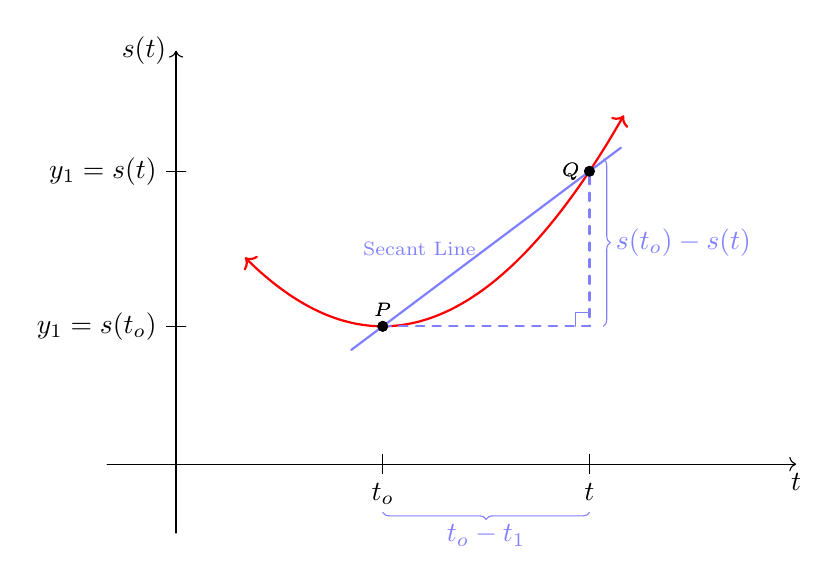
\begin{tikzpicture}[scale=1.75,cap=round]
        \tikzset{axes/.style={}}
        %\draw[style=help lines,step=1cm, dotted] (-5.25,-5.25) grid (5.25,5.25);
        % The graphic
        \begin{scope}[style=axes]
            \draw[->] (-.5,0) -- (4.5,0) node[below] {$t$};
            \draw[->] (0,-.5)-- (0,3) node[left] {$s(t)$};
            \foreach \x/\xtext in {1.5/t_{o}, 3/t}
            \draw[xshift=\x cm] (0pt,2pt) -- (0pt,-2pt) 
            node[below,fill=white,font=\normalsize]
            {$\xtext$};    
            \foreach \y/\ytext in {1/y_{1}=s(t_o), 2.125/y_{1}=s(t)}
            \draw[yshift=\y cm] (2pt,0pt) -- (-2pt,0pt) 
            node[left,fill=white,font=\normalsize]
      {$\ytext$};
      %%%
      \draw[domain=.5:3.25,smooth,variable=\x,red,<->,thick] plot ({\x},{.5*(\x-1.5)*(\x-1.5)+1});
      %%%
      \filldraw[black] (1.5,1) circle (1pt) node[above] {\scriptsize $P$};
      \filldraw[black] (3,2.125) circle (1pt) node[left] {\scriptsize $Q$};
      \draw[thick,blue!50,shorten >=-.5cm,shorten <=-.5cm] (1.5,1)--(3,2.125) 
      node[midway,left] {\scriptsize Secant Line};
      %%%
      \draw[blue!50,thick,dashed] (1.5,1)--(3,1)--(3,2.125);
      \draw[blue!50] (3,1.1)--(2.9,1.1)--(2.9,1);
      \draw[decoration={brace,mirror,raise=5pt},decorate,blue!50]
      (1.5,-.250) -- node[below=6pt] {$t_{o}-t_{1}$} (3,-.250);
      \draw[decoration={brace,mirror, raise=5pt},decorate,blue!50]
      (3,1) -- node[right=6pt] {$s(t_{o})-s(t)$} (3,2.215);
      %%%
      \filldraw[black] (1.5,1) circle (1pt) node[above] {\scriptsize $P$};
      \filldraw[black] (3,2.125) circle (1pt) node[left] {\scriptsize $Q$};
    \end{scope}
\end{tikzpicture}
\end{center}
\subsubsection{Instantaneous Velocity}
Instantaneous velocity is determined by computing average velocities over time interval $[t_o,t]$ that decrease in length. As $t$ approaches $t_0$, the $v_{avg}$ approaches the instantaneous velocity $v(t_0)$.
\begin{equation*}
    v(t_0)=\lim_{t\to t_0}\frac{s(t)-s(t_0)}{t-t_0}
\end{equation*}
\newpage

\subsubsection{Slope of the Tangent Line}
As we take the limit of $v_{avg}$ as $t$ approaches $t_0$, we get a tangent line. 
\begin{center}
    \begin{tikzpicture}[scale=2.5,cap=round,mark pos/.style args={#1/#2}{%
        postaction={decorate,decoration={markings,%
        mark=at position #1 with {
        \coordinate (#2);}}}}]
        \tikzset{axes/.style={}}
        %\draw[style=help lines,step=1cm, dotted] (-5.25,-5.25) grid (5.25,5.25);
        % The graphic
        \begin{scope}[style=axes]
          %%%
          \pgfmathsetmacro{\posP}{0.38}
         \draw[red,{Latex[bend]}-{Latex[bend]},thick,mark
         pos/.list={\posP-0.005/p-0,\posP/P,\posP+0.005/p-2,0.5/q-4,0.62/q-3,0.74/q-2,0.86/q-1}] plot[domain=.5:3.25,samples=101,variable=\x] ({\x},{.5*(\x-1.5)*(\x-1.5)+1});
         \draw[red] let \p1=($(p-2)-(p-0)$),\n1={(\y1/\x1)*(1cm/1pt)}
         in ($(P)-1*(1,\n1)$) -- ($(P)+2*(1,\n1)$) node[right,anchor=north
         west,font=\scriptsize,text width=1cm]{slope $m$ $=$ instantaneous velocity};
         \fill (P) circle (1pt) node[above,font=\scriptsize] {$P$};
         \foreach \X in {1,...,4}
         {\fill (q-\X) circle (1pt) node[below right,font=\scriptsize] {$Q_\X$};
         \path (P) -- (q-\X) coordinate[pos=-0.5] (L-\X) coordinate[pos={1.2+\X*0.3}] (R-\X);
         \draw[cyan,dashed] (L-\X) -- (R-\X) node[right,font=\scriptsize] (m\X) {slope $m_\X$}; }
         \draw[line width=2mm,-{Latex[bend]},red!20] ($(m1)+(0.5,0.1)$)
         to[out=-90,in=65] ++ (-0.2,-1.2);
          %%%
         %%%
        \end{scope}
        \end{tikzpicture}
\end{center}
We can define find the slope of the tangent line by finding the limit of the slope of the secant line as $t$ approaches $t_0$.
\begin{equation*}
    m(t_0)=\lim_{t\to t_0}\frac{s(t)-s(t_0)}{t-t_0}.
\end{equation*}

The limit defines the instantaneous velocity, therefore the instantaneous velocity at point $P$ of the graph is the slope of the tangent line at point $P$ of the position curve.   

There are parallels to the idea of limits. As $t\to 1$, the average velocity approaches the instantaneous velocity, just as the secant line approaches the tangent line.

\newpage
\section{Definitions of Limits}
\subsubsection{Defining the Limit of a Function (Preliminary)} 
The function $f$ is defined for all $x$ except possibly at $a$. If $f(x)$ is arbitrarily close to $L$ for all $x$ sufficiently close to $a$, then $f(x)$ is said to be \textbf{tending to $L$ as $x$ approaches $a$}. The limit of $f(x)$ as $x$ approaches $a$ is denoted by 
\begin{equation*}
    \lim_{x\to a}f(x)=L.
\end{equation*}
Often times the $\lim_{x\to a}f(x)=f(a)$, but this is not always the case and other methods for finding limits are available.

\subsubsection{Finding Limits from a Graph}

% Create a graph for demonstrating the idea of finding limits from a graph

\subsubsection{Finding Limits from a Table}
We create a table of values of a function corresponding to values of $x$ that are close to $a$.
\ex{}{
    \begin{center}
        Make a conjecture about $\lim_{x \to 1} \frac{\sqrt{x}-1}{x-1}$ using the tabular method.\\
        \begin{tabularx}{0.8\textwidth} { 
          | >{\raggedright\arraybackslash}X 
          | >{\centering\arraybackslash}X 
          | >{\centering\arraybackslash}X 
          | >{\centering\arraybackslash}X 
          | >{\centering\arraybackslash}X 
          | >{\centering\arraybackslash}X 
          | >{\centering\arraybackslash}X 
          | >{\centering\arraybackslash}X 
          | >{\raggedleft\arraybackslash}X | }
         \hline
         $x$ & $0.9$ & $0.99$ & $0.999$ & $0.9999$ & $1.0001$ & $1.001$ & $1.01$ & $1.1$ \\
         \hline
         $f(x)$ & $0.5132$ & $0.5013$ & $0.5001$ & $0.5000$ & $0.5000$ & $0.4999$ & $0.4988$ & $0.4881$  \\
        \hline
        \end{tabularx} \\
        We can make a mathematical conjecture that the $\lim_{x \to 1} \frac{\sqrt{x}-1}{x-1}=0.5$. 
    \end{center}
}

\subsubsection{One-Sided Limits}
The $\lim_{x \to a}  f(x)=L$ is referred to as two-sided limit because $f(x)$ approaches $L$ as $x$ approaches $a$ from both sides. However, there are times when we are only interested in the limit as $x$ approaches $a$ from one side. In this case, we use the notation $\lim_{x \to a^+}  f(x)=L$ or $\lim_{x \to a^-}  f(x)=L$ to denote the limit as $x$ approaches $a$ from the positive side or the negative side, respectively.

\subsubsection{Definition of One-Sided Limits}
\begin{enumerate}
    \item \underline{Right Sided Limits} Suppose $f$ is defined for all $x$ for all $x$ near $a$ with $x>a$. If $f(x)$ is arbitrarily close to $L$ for all $x$ sufficiently close to $a$ with $x>a$, we write,
    \begin{equation*}
        \lim_{x \to a^+}  f(x)=L.
    \end{equation*}
    \item \underline{Left Sided Limits} Analogously, suppose $f$ is defined for all $x$ for all $x$ near $a$ with $x<a$. If $f(x)$ is arbitrarily close to $L$ for all $x$ sufficiently close to $a$ with $x<a$, we write, 
    \begin{equation*}
        \lim_{x \to a^-}  f(x)=L.
    \end{equation*}
\end{enumerate}

\thm{}{The $\lim_{x \to a}  f(x)=L$ if and only if $\lim_{x \to a^-}  f(x)= \lim_{x \to a^+}f(x)= L$.}

\newpage
\section{Techniques for Computing Limits}
This section of the notes will cover the techniques for precisely computing the limits of functions without having the need to use mathematical evidence to create a conjecture.

\subsubsection{Limits of Linear Functions}
If $f(x)=mx+b$, then the $\lim_{x \to a}  f(x)=f(a)$. Linear functions allow for direct substitution of $x$ with $a$ to find the limit.

\thm{}{Let $a$,$b$ and $m$ be real numbers. For linear functions $f(x)=mx+b$, we have 
    \begin{equation*}
        \lim_{x \to a}  f(x)=ma+b.
    \end{equation*}
}

\subsubsection{Limit Laws}
\thm{Limit Laws}{
    \begin{enumerate}
        \item \underline{Sum Law} $\lim _{x \rightarrow a}(f(x)+g(x))=\lim _{x \rightarrow a} f(x)+\lim _{x \rightarrow a} g(x)$
        \item \underline{Difference Law} $\lim _{x \rightarrow a}(f(x)-g(x))=\lim _{x \rightarrow a} f(x)-\lim _{x \rightarrow a} g(x)$
        \item \underline{Constant Multiple Law} $\lim _{x \rightarrow a}(c f(x))=c \lim _{x \rightarrow a} f(x)$
        \item \underline{Product Law} $\lim _{x \rightarrow a}(f(x) g(x))=\left(\lim _{x \rightarrow a} f(x)\right)\left(\lim _{x \rightarrow a} g(x)\right)$
        \item \underline{Quotient Law} $\lim _{x \rightarrow a}\left(\frac{f(x)}{g(x)}\right)=\frac{\lim _{x \rightarrow a}(f(x)}{\lim _{x \rightarrow a} g(x)}, \text { provided } \lim _{x \rightarrow a} g(x) \neq 0$
        \item \underline{Power Law} $\lim _{x \rightarrow a}(f(x))^n=\left(\lim _{x \rightarrow a} f(x)\right)^n$
        \item \underline{Root Law} $\lim _{x \rightarrow a}(f(x))^{1 / n}=\left(\lim _{x \rightarrow a} f(x)\right)^{1 / n}, \text { provided } f(x)>0 \text {, for } x \text { near } a \text {, if } n \text { is even }$
    \end{enumerate}
}

\subsubsection{Limits of Polynomial Functions and Rational Functions}
The limit laws are used to find the limits of polynomial functions and rational functions. The limit of a polynomial function is found by direct substitution, $\lim_{x \rightarrow a} p(x)=p(a)$. And using the quotient limit law, we can find the limit of rational functions, 
\begin{equation*}
    \lim _{x \rightarrow a} \frac{p(x)}{q(x)}=\frac{\lim _{x \rightarrow a} p(x)}{\lim _{x \rightarrow a} q(x)}=\frac{p(a)}{q(a)}, \text { provided } q(a) \neq 0.
\end{equation*} 

\thm{Limits of Polynomial and Rational Functions}{
    \begin{enumerate}
    \item Polynomial functions: $\lim_{x \rightarrow a} p(x)=p(a)$
    \item Rational functions: $\lim _{x \rightarrow a} \frac{p(x)}{q(x)}=\frac{p(a)}{q(a)}, \text { provided } q(a) \neq 0$
    \end{enumerate}
}

\newpage

\subsubsection{One Sided Limits}
Theorem 1.3.1, 1.3.2, and 1.3.3 can be used to find the one-sided limits of functions. The one-sided limits are found by using the one-sided limit laws.

\thm{One Sided Limits}{
    Limit Laws 1-6 hold then the $\lim_{x \rightarrow a}$ replaced with $\lim_{x \rightarrow a^+}$ or $\lim_{x \rightarrow a^-}$. Law 7 is modified as follows. Assume $n >0$ is an integer. \\
    7. Root
a. $\lim _{x \rightarrow a^{+}}(f(x))^{1 / n}=\left(\lim _{x \rightarrow a^{+}} f(x)\right)^{1 / n}$, provided $f(x) \geq 0$, for $x$ near a with $x>a$, if $n$ is even
b. $\lim _{x \rightarrow a^{-}}(f(x))^{1 / n}=\left(\lim _{x \rightarrow a^{-}} f(x)\right)^{1 / n}$, provided $f(x) \geq 0$, for $x$ near a with $x<a$, if $n$ is even 
    
}

\subsubsection{Other Techniques for Computing Limits}
\begin{enumerate}
    \item Factor and cancel
    \item Use Conjugates
\end{enumerate}

\subsubsection{Squeeze Theorem}



% Module 2 Derivatives 
\newpage
\chapter{Module 02: Derivatives}
\section{Introducing the Derivative}
The problem that was introduced in Chapter 2 about finding the slope of the tangent is important for several reasons.
\begin{itemize}
    \item We identify the slope of the tangent line with the \emph{instantaneous rate of change} of a function.
    \item The slopes of the tangent line as they change along a curve are the values of a new function called the \emph{derivative}.
    \item If a curve represents the trajectory of a moving object, the tangent line at a point on the curve indicates the direction of the motion at that point.
\end{itemize}

The instantaneous velocity at time $t=a$ is the limit of the average velocity as $t \rightarrow a$:
\begin{equation*}
    v_{inst}=\lim_{t \to a} \frac{s(t) -s(a)}{t-a}
\end{equation*}

We also learned that there are special geometric meanings to these quantities. The average velocity is the slope of the secant line and the instantaneous velocity is the slope of the tangent line.

\subsubsection{Tangent lines and Rates of Change}
Consider the curve $y=f(x)$ and a secant line intersecting the curve at points $P(a,f(a))$ and $Q(x,f(x))$. The difference $f(x_-f(a)$ is the change in the value of $f$ on the interval $[a,x]$, while $x-a$ is the change in $x$. As discussed before the slope of the secant line $\overleftrightarrow{PQ}$, is the $\lim_{x \to a }\frac{f(x)-f(a)}{x-a}$
\begin{center}
    \begin{tikzpicture}[scale=2.5,cap=round,mark pos/.style args={#1/#2}{%
        postaction={decorate,decoration={markings,%
        mark=at position #1 with {
        \coordinate (#2);}}}}]
        \tikzset{axes/.style={}}
        %\draw[style=help lines,step=1cm, dotted] (-5.25,-5.25) grid (5.25,5.25);
        % The graphic
        \begin{scope}[style=axes]
          %%%
          \pgfmathsetmacro{\posP}{0.38}
         \draw[red,{Latex[bend]}-{Latex[bend]},thick,mark
         pos/.list={\posP-0.005/p-0,\posP/P,\posP+0.005/p-2,0.5/q-4,0.62/q-3,0.74/q-2,0.86/q-1}] plot[domain=.5:3.25,samples=101,variable=\x] ({\x},{.5*(\x-1.5)*(\x-1.5)+1});
         \draw[red] let \p1=($(p-2)-(p-0)$),\n1={(\y1/\x1)*(1cm/1pt)}
         in ($(P)-1*(1,\n1)$) -- ($(P)+2*(1,\n1)$) node[right,anchor=north
         west,font=\scriptsize,text width=1cm]{slope $m$ $=$ instantaneous velocity};
         \fill (P) circle (1pt) node[above,font=\scriptsize] {$P$};
         \foreach \X in {1,...,4}
         {\fill (q-\X) circle (1pt) node[below right,font=\scriptsize] {$Q_\X$};
         \path (P) -- (q-\X) coordinate[pos=-0.5] (L-\X) coordinate[pos={1.2+\X*0.3}] (R-\X);
         \draw[cyan,dashed] (L-\X) -- (R-\X) node[right,font=\scriptsize] (m\X) {slope $m_\X$}; }
         \draw[line width=2mm,-{Latex[bend]},red!20] ($(m1)+(0.5,0.1)$)
         to[out=-90,in=65] ++ (-0.2,-1.2);
          %%%
         %%%
        \end{scope}
        \end{tikzpicture}
\end{center}

\newpage

\subsubsection{Definition Rate of Change and the Slope of the Tangent Line}

The \textbf{average rate of change} in $f$ on the interval $[a,x]$ is the corresponding secant line:
\begin{equation*}
    m_{sec}=\frac{f(x)-f(a)}{x-a}
\end{equation*}

The \textbf{instantaneous rate of change } in $f$ at $a$ is 
\begin{equation*}
    m_{tan}=\lim_{x \to a } \frac{f(x)-f(a)}{x-a}
\end{equation*}

which is also the slope of the tangent line at $(a,f(a)$ provided that the limit exists. Tangent line through $(a,f(a))$ with slope $m_{tan}$. Its equation is

\begin{equation*}
    y-f(a)=m_{tan}(x-a)
\end{equation*}

\subsubsection{Alternative Definition Rate of Change and the Slope of the Tangent Line}
The \textbf{average rate of change} in $f$ on the interval $[a, a +h]$ is the slope of the corresponding secant line:

\begin{equation*}
    m_{sec}=\frac{f(a+h)-f(a)}{h}
\end{equation*}

The \textbf{instantaneous rate of change} in $f$ at $a$ is 

\begin{equation*}
    m_{tan}=\lim_{h \to 0} \frac{f(a+h)-f(a)}{h}
\end{equation*}

\subsubsection{The Derivative}
Computing the slope of the line tangent to the graph of a function $f$ at a point $a$ gives us the instantaneous  rate of change in $f$ at $a$. This is called the derivative.

The \textbf{derivative of $f$ at $a$} written,

\begin{equation*}
    f`(a)=\lim_{h \to 0} \frac{f(a+h)-f(a)}{h}
\end{equation*}

\newpage
\section{Derivative as a Function}
In this section we now extend our understandings of derivatives to all points in the domain $f$ to create new function called the derivative of $f$.


\subsubsection{The Derivative Function}
Due to the fact that the tangent of any given function moves, the slope of the tangent line will also change. For this reason, the slope on the tangent line for the function $f$ is itself a function, call the \emph{derivative} of $f$.


\begin{center}
    \begin{tikzpicture}
        % Axes
        \draw [->, name path=x] (-1,0) -- (11,0) node [right] {$x$};
        \draw [->] (0,-1) -- (0,6) node [above] {$y$};
        % Origin
        \node at (0,0) [below left] {$0$};
        % Points
        \coordinate (start) at (1,-0.8);
        \coordinate (c1) at (3,3);
        \coordinate (c2) at (5.5,1.5);
        \coordinate (c3) at (8,4);
        \coordinate (end) at (10.5,-0.8);
        % show the points
        \foreach \n in {start,c1,c2,c3,end} \fill [black] (\n)
            circle (2pt) node [below] {};
        % join the coordinates
        \draw [thick,name path=curve] (start) to[out=70,in=180] (c1) to[out=0,in=180]
            (c2) to[out=0,in=180] (c3) to[out=0,in=150] (end);
        % add tangets and dashed lines
        \foreach \c in {1,2,3} {
            %\draw [dashed] let \p1=(c\c) in (c\c) -- (\x1,0) node [below] {$c_\c$};
            \draw ($(c\c)-(0.75,0)$) -- ($(c\c)+(0.75,0)$) node [midway,above=4mm]{}; %{$f'(c_\c)=0$};
        }
        % add a and b
        \path [name intersections={of={x and curve}, by={a,b}}] 
            (a) node [below left] {$a$}
            (b) node [above right] {$b$};
            
        \DrawTangent[red, thick]{curve}{-1}{4}{1.5}
        \DrawTangent[orange, thick]{curve}{-1}{4}{3.5}
        
        \end{tikzpicture}
\end{center}

\subsubsection{Definition The Derivative Function}
The \textbf{derivative} $f$ is the function

\begin{equation*}
    f'(x)=\lim_{h \to 0} \frac{f(x+h)-f(x)}{h}
\end{equation*}

provided the limit exists and $x$ is in the domain $f$.

\ex{Find the derivative of $f(x)=-x^2+6x$}{
    \begin{align*}
        f'(x) & = \lim_{h \to 0} \frac{f(x+h)- f(x)}{h} \\
        & = \lim_{h \to 0} \frac{-(x+h)^2 +6(x+h)-(-x^2+6x)}{h} \\
        & = \lim_{h \to 0} \frac{-(x^2+2xh+h^2)+6x+6h+x^2-6x}{h} \\
        & = \lim_{h \to 0} \frac{h(-2x-h+6)}{h} \\
        & = \lim_{h \to 0} (-2x-h+6)\\
        & = \boxed{-2x+6} 
    \end{align*}
}

\newpage

\subsubsection{Derivative Notation}
Several notations for the derivatives are used. Recall the equation for the slope of the secant line,

\begin{equation*}
    m_{sec}=\frac{f(x + \Delta x)-f(x)}{\Delta x} = \frac{\Delta y}{\Delta x}
\end{equation*}

By letting $\Delta x \to 0$, the slope of the tangent line at $(x,f(x))$ is 

\begin{equation*}
    f'(x)=\lim_{\Delta x \to 0} \frac{(f(x+ \Delta x)- f(x))}{\Delta x}= \lim_{\Delta x \to 0} \frac{\Delta y}{\Delta x }= \frac{dy}{dx}
\end{equation*}

\subsubsection{Continuity}
If a function is differentiable at a point, then it is also continuous at that point.

\thm{Differentiable Implies Continuous}{If $f$ is differentiable at $a$, then $f$ is continuous $a$.}

\subsubsection{When Is a Function Not Differentiable at a Point?}
A function $f$ is not differentiable at $a$ if at least one of the following conditions hold:

\begin{enumerate}
    \item $f$ is not continuous at $a$
    \item $f$ has a corner at $a$
    \item $f$ has a vertical tangent at $a$
\end{enumerate}


\newpage

\section{Rules of Differentiation}
If we had to constantly use limits in order to evaluate derivatives, then calculus would be very tedious. In this section of the notes, we will establish rules and formulas for calculating derivatives quickly.

\subsubsection{The Constant and Power Rules for Derivatives}
The graph of the \textbf{constant function} $f(x)=c$ is a horizontal line with a slope of zero at every point. Which leads us to the following theorem.

\thm{Constant Rule}{If $c$ is a real number, then $\frac{d}{dx}(c) =0$.}

Now, we consider the functions of the form $f(x)=x^n$, where $n$ is a non negative integer. When evaluating the derivatives of the said, form, using limits we find that the derivative of $x^n$ could be evaluated by placing the exponent $n$ in front of $x$ as a coefficient and decreasing the exponent by $1$. Using these observations, we state the theorem. 

\thm{Power Rule}{If $n$ is a non-negative integer, then $\frac{d}{dx}(x^n)=nx^{n-1}$.}

\subsubsection{Constant Multiple Rule}

We find the derivative of a constant multiple $c$ multiplied by a function $f$. 
\begin{align*}
        \frac{d}{dx}(cf(x)) & = \lim_{h \to 0 } \frac{cf(x+h) - cf(x)}{h} \\
        &= \lim_{h \to 0 } \frac{c(f(x+h) - f(x))}{h} \\
        &= c\lim_{h \to 0 } \frac{f(x+h) - f(x)}{h} \\
        & = cf'(x)
\end{align*}

\thm{Constant Multiple Rule}{If $f$ is differentiable at $x$ and $c$ is a constant, then 
\begin{equation*}
    \frac{d}{dx}(cf(x))= cf'(x)
\end{equation*}}

\subsubsection{Sum Rule}
Many functions are sums of simpler functions. Therefore, it makes it very convenient if we were to establish  a rule for calculating the derivative of the sum of two or more functions. 

\thm{Sum Rule }{If $f$ and $g$ are differentiable at $x$, then 
\begin{equation*}
    \frac{d}{dx} (f(x)+g(x))= f'(x) + g'(x)
\end{equation*}}

The sum rule can be extended to three or more differentiable functions $f_1$, $f_2$, $\ldots$, $f_n$, to obtain the \textbf{Generalized Sum Rule}:

\begin{equation*}
    \frac{d}{dx} (f_1(x) + f_2(x) + \ldots + f_n(x)) =  f'_1(x) + f'_2(x) + \ldots + f'_n(x).
\end{equation*}

\subsubsection{The Derivative of the Natural Exponential Function}
We come to the fact that

\begin{equation*}
    \lim_{h \to 0} \frac{e^h - 1}{h}= 1
\end{equation*}
(The proof of this is found in Page 157 of the textbook and I will not write it here).

With the preceding facts in mind, the derivative of $f(x) = e^x$ is computed as follows:

\begin{align*}
    \frac{d}{dx}(e^x) &= \lim_{h \to 0} \frac{e^{x+h} - e^x}{h} \\
    &= \lim_{h \to 0} \frac{e^x + e^h - e^x}{h} \\
    &= \lim_{h \to 0} \frac{e^x(e^h- 1)}{h}  \\
    &= e^x \cdot \lim_{h \to 0} \frac{e^h- 1}{h} \\
    &= e^x \cdot 1 = e^x.
\end{align*}

\thm{Derivative of $e^x$}{The functions $f(x)= e^x$ is differentiable for all real number $x$, and 
\begin{equation*}
    \frac{d}{dx} (e^x) =e^x
\end{equation*}
} 

\subsubsection{Higher-Order Derivatives}
Because the derivative of a function $f$ is a function in its own right, we can take the derivative $f'$. The result is the \emph{second derivative of $f$}, denoted $f''$. The derivative of the second derivative is the \emph{third derivative of $f$}, denoted by $f'''$. In general, derivatives of order $n \ge 2$ are called \emph{higher-order derivatives}.

Other common notations for the second derivative of $y=f(x)$ include $\frac{d^2y}{dx^2}\frac{d^2f}{dx^2}$; the notations $\frac{d^ny}{dx^n}\frac{d^nf}{dx^n}$, are used for the $n$th derivative of $f$.


% \chapter{Module 03: More Derivatives}
% \chapter{Module 04: Midterm Exam}
% \chapter{Module 05: Applications of Derivatives}
% \chapter{Module 06: L'Hopital's Rule and Integration}
% \chapter{Module 07: Applications of Integration}
% \chapter{Module 08: Final Exam}


\end{document}
